% ===========================================================================
\section{Pilot Study}
\label{sec:pilot}
% ===========================================================================

The pilot asks three questions of the smallest models that can answer them.
Does a model trained on textbooks read them or memorise them (E1)?
Which exercise types must be in the training set for which abilities to appear (E2)?
Does re-applying the same layers extend the chain of rules a model can follow (E3)?
A fourth experiment (E4) isolates an effect of the training distribution that we ran into while designing the benchmark.


\paragraph{Setup.}
All models are decoder-only transformers of width 64 with four attention heads.
The default model applies a block of two layers twice, for four layer passes and \NparamsMain{} parameters.
Training takes 5{,}000 steps of 32 episodes (8{,}000 steps in E3) on one CPU core, which is between \MinRunMinutes{} and \MaxRunMinutes{} minutes per run.
Accuracy is measured on 4{,}000 held-out episodes per test, giving a standard error below 0.8 percentage points.
Appendix~\ref{app:details} gives the remaining details, and Appendix~\ref{app:runs} lists every run.
The pilot comprises \TotalRuns{} runs and \TotalCpuHours{} CPU-hours.
The number of seeds per condition is small and is stated with each result; we therefore describe only effects that are large compared with the gap between the guessing level and ceiling.

\subsection{E1: Memorising a textbook versus reading one}

Every training episode draws its textbook from a fixed pool of $M$ textbooks, or from an unlimited supply ($M=\infty$).
The exercises are sampled afresh each time, half of them \skill{follow} and half \skill{compose} at depth 2, and the number of training episodes is the same for every $M$.
We then test on textbooks from the pool (G0) and on new textbooks (G1).

\begin{table}[t]
\centering\small
\begin{tabular}{@{}lcccc@{}}
\toprule
Distinct textbooks & \multicolumn{2}{c}{G0: seen textbooks} & \multicolumn{2}{c}{G1: new textbooks} \\
\cmidrule(lr){2-3}\cmidrule(lr){4-5}
in training ($M$) & \skill{follow} & \skill{compose}-2 & \skill{follow} & \skill{compose}-2 \\
\midrule
1 & 100.0 & 100.0 & 20.7 & 21.3 \\
4 & 100.0 & 100.0 & 22.8 & 21.2 \\
16 & 100.0 & 100.0 & 31.4 & 21.1 \\
64 & 100.0 {\scriptsize\,2/2} & 99.8 {\scriptsize\,2/2} & 90.5 {\scriptsize\,1/2} & 51.3 {\scriptsize\,0/2} \\
$\infty$ & 100.0 {\scriptsize\,2/2} & 100.0 {\scriptsize\,2/2} & 100.0 {\scriptsize\,2/2} & 100.0 {\scriptsize\,2/2} \\
\bottomrule
\end{tabular}

\caption{E1: accuracy (\%) after training on $M$ distinct textbooks. One seed for $M \le 16$; for $M = 64$ and $M = \infty$ the mean of two seeds, followed by the number of seeds that ended at 95\% or above. On new textbooks the guessing level is 20\% for \skill{follow} and \GuessTwo\% for \skill{compose}-2. Seen textbooks tabulate arbitrary maps, as in training; new textbooks tabulate permutations.}
\label{tab:e1}
\end{table}

\begin{figure}[t]
\centering
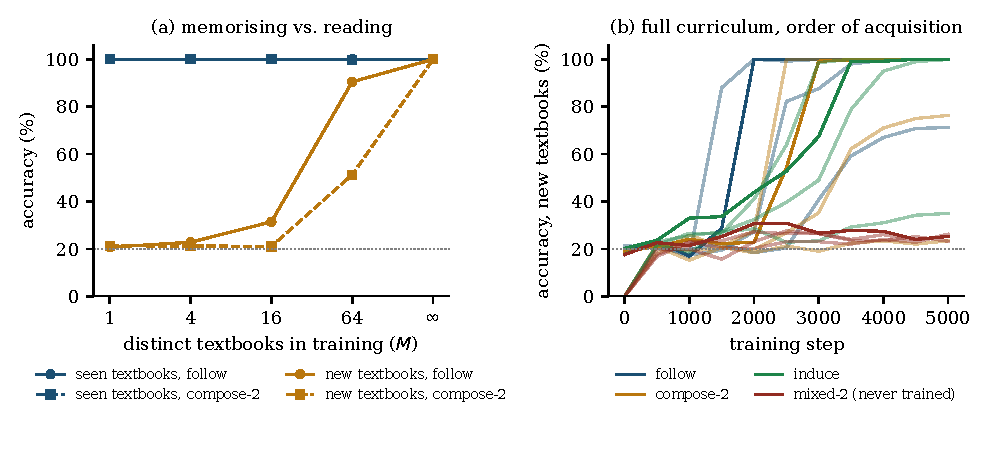
\includegraphics[width=\linewidth]{gen/fig_e1_e2.pdf}
\caption{\textbf{(a)} E1 (means over seeds). All models answer almost perfectly on their training textbooks; only those trained on enough distinct textbooks can use a new one. \textbf{(b)} E2, full curriculum, accuracy on new textbooks during training for each seed (later seeds are drawn lighter). The skills are acquired one after another in abrupt steps, and the never-trained combination \skill{mixed} stays at the guessing level. Dotted line: 20\%.}
\label{fig:e1e2}
\end{figure}

Table~\ref{tab:e1} and Figure~\ref{fig:e1e2}a show the outcome.
Every model answers exercises about its training textbooks almost perfectly.
For $M \le 16$ that is all it can do: on a new textbook, \skill{follow} accuracy is \EOneMOneNewFollow\%, \EOneMFourNewFollow\% and \EOneMOneSixNewFollow\% for $M = 1, 4, 16$.
These models have stored their textbooks in the weights and do not consult the page in front of them.
With $M = 64$ the same architecture, trained for the same number of steps, begins to use textbooks it has never seen: over two seeds it follows their rules at \EOneMSixFourNewFollowList\% and composes them at \EOneMSixFourNewComposeTwoList\%.
With an unlimited supply, both seeds reach at least \EOneMInfNewFollowMin\% on \skill{follow} and \EOneMInfNewComposeTwoMin\% on \skill{compose}.

The switch from memorising to reading as the number of distinct textbooks grows is the instructional-material counterpart of the task-diversity threshold reported for in-context regression \citep{raventos2023diversity} and for modular arithmetic \citep{he2024grok}.
Four points are worth drawing out.

\emph{Accuracy on seen material is uninformative.}
The G0 columns are the same, to within half a point, for models that read and models that do not.
Any evaluation in which the rules were available during training, in whatever form, cannot distinguish the two.

\emph{Variety made the difference, not volume.}
Every model saw the same 160{,}000 training episodes.
What changed is how many different textbooks those episodes were about.
This is the first half of hypothesis H3 in Section~\ref{sec:protocol}.

\emph{The harder skill asks for more variety.}
At $M=64$, \skill{follow} transfers to new textbooks largely or completely (\EOneMSixFourNewFollowList\%) while \skill{compose} lags behind (\EOneMSixFourNewComposeTwoList\%).
With one or two seeds per condition we do not read more into the location of the threshold than that reading begins somewhere between 16 and 64 textbooks for the easier skill and is not complete at 64 for the harder one.

\emph{Knowledge in the weights did not help with a new page.}
The models with $M \le 16$ know their textbooks perfectly and are at or near chance on a new one.
This bears on hypothesis H2 only indirectly: the direct test, adding facts to the weights of a model that already reads, is left to the full-scale study.



\subsection{E2: Which skills have to be trained}

We train four models on new textbooks only ($M=\infty$): one on all three exercise types in equal proportion, and three with one type left out and the remaining two in equal proportion.
\skill{compose} is trained at depth 2 only.
All four are tested on the three trained types and on two G2 tests: \skill{mixed} at depth 2, which combines \skill{compose} with \skill{induce}, and \skill{compose} at depth 3.

\begin{table}[t]
\centering\small
\begin{tabular}{@{}lccccc@{}}
\toprule
& \multicolumn{3}{c}{G1: exercise types in the curriculum} & \multicolumn{2}{c}{G2: never trained} \\
\cmidrule(lr){2-4}\cmidrule(lr){5-6}
Training set & \skill{follow} & \skill{compose}-2 & \skill{induce} & \skill{mixed}-2 & \skill{compose}-3 \\
\midrule
Full curriculum & 92.8 {\scriptsize\,3/4} & 74.9 {\scriptsize\,2/4} & 83.7 {\scriptsize\,3/4} & 25.0 {\scriptsize\,0/4} & 20.5 {\scriptsize\,0/4} \\
without \skill{follow} & 19.7 {\scriptsize\,0/4} & 25.3 {\scriptsize\,0/4} & 81.4 {\scriptsize\,2/4} & 22.0 {\scriptsize\,0/4} & 21.1 {\scriptsize\,0/4} \\
without \skill{compose} & 73.8 {\scriptsize\,2/4} & 19.5 {\scriptsize\,0/4} & 99.8 {\scriptsize\,4/4} & 20.0 {\scriptsize\,0/4} & 20.5 {\scriptsize\,0/4} \\
without \skill{induce} & 100.0 {\scriptsize\,4/4} & 100.0 {\scriptsize\,4/4} & 20.4 {\scriptsize\,0/4} & 17.0 {\scriptsize\,0/4} & 20.4 {\scriptsize\,0/4} \\
\bottomrule
\end{tabular}

\caption{E2: accuracy (\%) on new textbooks after training with one exercise type left out. Each cell gives the mean over seeds, followed by the number of seeds that ended at 95\% or above out of the number run. Guessing levels: 20\% for \skill{follow}, 25\% for \skill{induce}, \GuessTwo\% for \skill{compose}-2, \GuessThree\% for \skill{compose}-3, and 26.7\% on \skill{mixed}-2 for a model that has induced $g$ but cannot combine it with a table look-up (see text).}
\label{tab:e2}
\end{table}

Table~\ref{tab:e2} gives the result, and the first thing it shows is how uneven learning is at this budget.
Skills are acquired in abrupt steps (Figure~\ref{fig:e1e2}b), so a run ends either near ceiling or near chance, and whether a given step arrives before training stops varies with the seed.
Even \skill{follow}, the simplest skill, was solved in only \ETwoPoolFollowTrainedSolved{} of the \ETwoPoolFollowTrainedRuns{} runs whose training set contained it.
Alongside each mean we therefore report how many seeds ended at 95\% or above, and we read the table by comparing those counts.

\paragraph{A skill left out of training was never acquired.}
Without \skill{induce} exercises, \skill{induce} accuracy is at or below its guessing level in every seed (\ETwoNoInduceInduceList\%); without \skill{compose} exercises, so is \skill{compose} (\ETwoNoComposeComposeTwoList\%).
Following and composing do not yield induction, and following and inducing do not yield composition.
Within TinyTextbook each skill is therefore necessary for itself, which is the minimality condition of Section~\ref{sec:ladder} at level G1.

\paragraph{Leaving out the simplest skill removed more than that skill.}
The models trained on \skill{compose} and \skill{induce}, but never on a single look-up, did not learn to look up (\ETwoNoFollowFollowList\% on \skill{follow}) and did not learn to compose either (\ETwoNoFollowComposeTwoList\%, which is the guessing level for two-step chains).
\skill{compose} was solved in \ETwoPoolComposeWithoutFollowSolved{} of \ETwoPoolComposeWithoutFollowRuns{} runs without \skill{follow} in the training set, against \ETwoPoolComposeWithFollowSolved{} of \ETwoPoolComposeWithFollowRuns{} runs with it (the full curriculum and the one without \skill{induce}; one-sided Fisher exact test, $p = \ETwoFisherP$).
A two-step exercise contains two look-ups, so in principle it supervises everything a one-step exercise does.
In practice the one-step exercise acted as a stepping stone without which the two-step skill was not found within the budget.
This also answers, for this benchmark, the worry raised in Section~\ref{sec:curriculum} that rule following cannot be removed separately from composition: it can, and removing it matters.

\paragraph{The full curriculum was not learned in every seed.}
With all three exercise types in training, \ETwoFullFollowSolved{} of \ETwoFullSeeds{} seeds solved \skill{follow}, \ETwoFullComposeTwoSolved{} solved \skill{compose} and \ETwoFullInduceSolved{} solved \skill{induce}; \ETwoFullAllSolved{} solved all three.
Across all conditions, the runs that fell short either made their first transition late, when the learning rate had already decayed too far for the remaining skills to follow, or never made it.
Nothing in our data explains which seeds these are.
The practical consequence is that a leave-one-out comparison at a fixed budget must be read through counts over seeds, as above, and Section~\ref{sec:protocol} lists the corrections we would make to the design.


\paragraph{Trained skills did not combine by themselves.}
\skill{mixed} exercises ask for a tabulated function and the induced function in one chain.
The models trained on the full curriculum score \ETwoFullMixedTwo\% on them (per seed: \ETwoFullMixedTwoList).
This is no better than guessing: when $g$ is the outer function, its input cannot be one of the two example keys, so the answer is one of three symbols that the examples determine, and when $g$ is the inner function the answer is uniform; a model that has induced $g$ and otherwise guesses therefore reaches $(1/3 + 1/5)/2 = 26.7\%$.
None of the \ETwoRunsAll{} runs in this experiment solved \skill{mixed}; the best reached \ETwoMixedMax\%.
Having each skill in the weights was not enough to obtain their combination, which contradicts hypothesis H5 at this scale.
\skill{compose} at depth 3 is likewise at its guessing level in every run, as expected from four layer passes trained on two-step chains; E3 examines depth directly.



\subsection{E3: Recurrent depth}

All models in this experiment are trained on \skill{compose} exercises whose chain length is 1, 2, 3 or 4 with equal probability (length 1 is \skill{follow}), and are tested at lengths 1 to 6.
We compare a block of two layers applied once, twice and three times with unshared stacks of four and six layers.
A looped model with $r$ loops and an unshared model with $2r$ layers perform the same number of layer passes, and the looped one has $1/r$ of the transformer-block parameters.

\begin{table}[t]
\centering\small
\begin{tabular}{@{}lccccccccc@{}}
\toprule
& & Layer & & \multicolumn{4}{c}{G1: chain lengths in training} & \multicolumn{2}{c}{G2: longer} \\
\cmidrule(lr){5-8}\cmidrule(lr){9-10}
Model & Params & passes & Seeds & 1 & 2 & 3 & 4 & 5 & 6 \\
\midrule
2 layers $\times$ 1 loop & 113k & 2 & 1 & 100.0 & 24.9 & 24.4 & 22.9 & 21.4 & 22.1 \\
2 layers $\times$ 2 loops & 113k & 4 & 3 & 100.0 {\scriptsize\,3/3} & 100.0 {\scriptsize\,3/3} & 71.9 {\scriptsize\,1/3} & 23.4 {\scriptsize\,0/3} & 22.2 {\scriptsize\,0/3} & 21.8 {\scriptsize\,0/3} \\
2 layers $\times$ 3 loops & 113k & 6 & 1 & 100.0 & 100.0 & 46.7 & 23.2 & 23.0 & 22.3 \\
4 layers, unshared & 213k & 4 & 3 & 100.0 {\scriptsize\,3/3} & 89.3 {\scriptsize\,1/3} & 55.0 {\scriptsize\,1/3} & 31.3 {\scriptsize\,0/3} & 21.6 {\scriptsize\,0/3} & 21.8 {\scriptsize\,0/3} \\
6 layers, unshared & 313k & 6 & 1 & 100.0 & 95.2 & 65.1 & 25.1 & 22.1 & 22.8 \\
\bottomrule
\end{tabular}

\caption{E3: accuracy (\%) on new textbooks by chain length. Where a model has several seeds, the mean is followed by the number of seeds that ended at 95\% or above out of the number run. Guessing levels for lengths 1 to 6: \GuessOne, \GuessTwo, \GuessThree, \GuessFour, \GuessFive{} and \GuessSix\%.}
\label{tab:e3}
\end{table}

\begin{figure}[t]
\centering
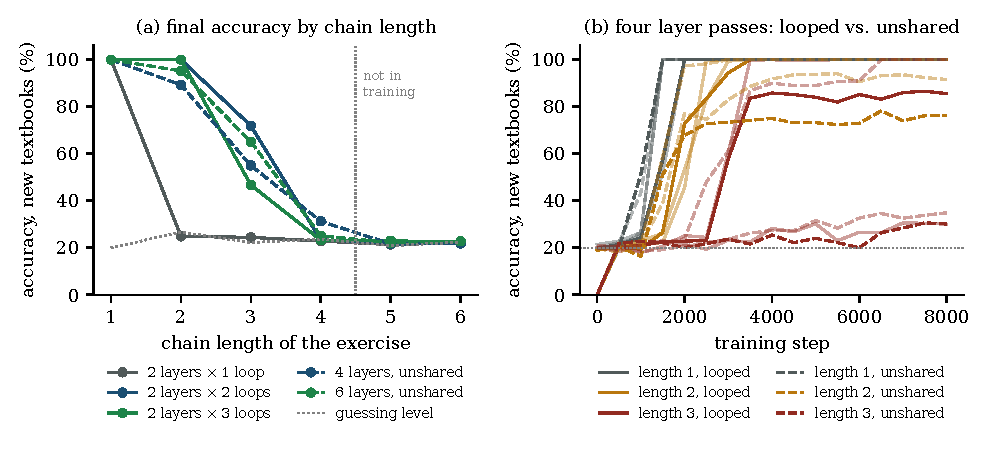
\includegraphics[width=\linewidth]{gen/fig_e3.pdf}
\caption{E3. \textbf{(a)} Final accuracy by chain length, averaged over seeds; solid lines are looped models, dashed lines unshared ones, colour marks the number of layer passes, and the dotted grey curve is the guessing level. \textbf{(b)} Accuracy during training for the two models with four layer passes, one curve per seed (later seeds lighter). The chain lengths are acquired one after another, at times that differ widely between seeds. Dotted horizontal line: 20\%.}
\label{fig:e3}
\end{figure}

\paragraph{Loops supplied depth without adding parameters.}
With two layer passes the model learned single look-ups and nothing longer (\EThreeTiedTwoXOneDepthTwo\% at length 2, below the guessing level; one seed).
Applying the same two layers a second time, with not one parameter added, was enough for length 2 to be solved in all \EThreeTiedTwoXTwoSeeds{} seeds and for length 3 to reach \EThreeTiedTwoXTwoDepthThree\% on average (per seed: \EThreeTiedTwoXTwoDepthThreeList).
This is hypothesis H4 as stated in Section~\ref{sec:protocol}: at a fixed parameter count, a second loop raised the chain length the model could follow.

\paragraph{At equal depth, looped and unshared models showed no consistent difference.}
The unshared four-layer model has the same number of layer passes as the two-loop model and \EThreeUntiedFourParams{} parameters instead of \EThreeTiedTwoXTwoParams.
Over \EThreeTiedTwoXTwoSeeds{} seeds each, accuracy at length 2 was \EThreeTiedTwoXTwoDepthTwoList\% for the looped model and \EThreeUntiedFourDepthTwoList\% for the unshared one; at length 3 it was \EThreeTiedTwoXTwoDepthThreeList\% and \EThreeUntiedFourDepthThreeList\%; and at length 4, \EThreeTiedTwoXTwoDepthFourList\% and \EThreeUntiedFourDepthFourList\%.
The looped model was ahead at length 2 in two seeds and at length 3 in one; the unshared model was ahead in another seed, the only run in the experiment to rise clearly above the guessing level at length 4.
The spread between seeds is as large as any difference between the architectures (Figure~\ref{fig:e3}b), and with three seeds we do not claim a difference in either direction.
What can be said is the weaker statement that sharing weights across depth cost nothing measurable here while halving the number of block parameters.
Earlier work reports that weight sharing favours iterative computation \citep{yang2024looped,saunshi2025latent}; our data neither confirm nor contradict this at equal depth.


\paragraph{A third loop made no visible difference.}
The three-loop model learned length 2 completely and reached \EThreeTiedTwoXThreeDepthThree\% at length 3, which is inside the range spanned by the two-loop seeds (one seed).
In an exploratory run with a longer schedule of 10{,}000 steps the same model reached 95\% at length 3 by step 6{,}500.
We therefore have no evidence that a third loop helps and none that it hurts; the question needs more seeds and a longer budget than we had.

\paragraph{No model went beyond the lengths it was trained on.}
Accuracy at lengths 5 and 6 is at the guessing level for every model and every seed, including the models with six layer passes.
Like the \skill{mixed} test of E2, this is a failure at level G2.


\subsection{E4: A symmetric training distribution holds the reading skill back}
\label{sec:symmetry}

Our first training sets tabulated permutations, as the test sets do, and in exploratory runs the models did not learn to look a value up (Appendix~\ref{app:negative}).
E4 examines this in isolation.
Two groups of models are trained on \skill{follow} exercises only, with identical settings except for one: in one group the tabulated functions of the training textbooks are arbitrary maps, in the other they are permutations.
Both groups are tested on new textbooks of both kinds.

\begin{table}[t]
\centering\small
\begin{tabular}{@{}lcccc@{}}
\toprule
Tables in & & \multicolumn{2}{c}{\skill{follow} on new textbooks with} & First checkpoint \\
\cmidrule(lr){3-4}
training & Seeds & permutations & arbitrary maps & at $\ge 95\%$ (per seed) \\
\midrule
Arbitrary maps & 3 & 100.0 {\scriptsize\,3/3} & 100.0 {\scriptsize\,3/3} & 1{,}500, 2{,}000, 2{,}500 \\
Permutations & 3 & 38.7 {\scriptsize\,0/3} & 31.6 {\scriptsize\,0/3} & never, never, never \\
\bottomrule
\end{tabular}

\caption{E4: \skill{follow} accuracy (\%) after training on \skill{follow} only, with training tables that are arbitrary maps or permutations. Mean over seeds, followed by the number of seeds that ended at 95\% or above out of the number run. The last column gives, per seed, the first of the checkpoints (taken every 500 steps) at which accuracy on new permutation textbooks was at least 95\%. The guessing level is 20\% on permutation textbooks; on textbooks of arbitrary maps a model can exceed it by guessing a frequent symbol.}
\label{tab:e4}
\end{table}

Table~\ref{tab:e4} shows the result.
With arbitrary maps in training, all \EFourTrainMapsSeeds{} seeds made an abrupt transition from chance to ceiling (first at 95\% or above at steps \EFourTrainMapsFirst) and ended at 100\% on both kinds of new textbook.
With permutations in training, no seed made that transition within 5{,}000 steps: accuracy crept above chance during the second half of training and ended at \EFourTrainPermsFollowPermList\% on new permutation textbooks.
The comparison is tilted against the first group, which is tested on tables from a different distribution than the one it was trained on, while the second group is tested on its own training distribution; the group with the distribution shift is the one that learned.


Our explanation, which we have not tested directly, is the following.
When every row is a permutation, the multiset of symbols in a row is the same in every episode, so an attention pattern that spreads over a row, or over the whole table, carries no information about the answer; only attention concentrated on the single correct cell does, and from a diffuse start there is little gradient leading towards it.
When rows are arbitrary maps, the symbols that occur more often in row $j$ are more likely to be the answer to a question about $f_j$, so attending to the right row already lowers the loss, and from there the model can sharpen onto the right cell.
If this account is correct, it is a statement about curriculum design: a reading skill may be learnable in practice only when the training distribution also rewards a cruder version of it.


\subsection{What did not work}
\label{sec:negative}

\paragraph{Retrieval by content was not learned within our budget.}
In the shuffled layout a value must be found by matching the function name and the key against free-standing facts.
In exploratory runs (Appendix~\ref{app:negative}; single seeds, not controlled comparisons), \skill{follow} stayed at chance in that layout with permutations and with arbitrary maps, for as long as we trained (between 1{,}500 and 4{,}000 steps, depending on the run).
The aligned layout replaces retrieval by content with retrieval by address, and all results in this paper are for that easier setting.
Retrieval by key is part of layer C1, so the pilot leaves the hardest primitive of the proposed curriculum untested.

\subsection{Where the pilot leaves the hypotheses}

Table~\ref{tab:summary} sets the pilot against the five hypotheses of Section~\ref{sec:protocol}.
H1 to H4 were written down before any experiment was run.
H1 is given in the form to which the pilot led us to narrow it: originally it predicted that removing rule following would lower accuracy on \emph{every} exercise type, whereas \skill{induce}, which in TinyTextbook needs no table look-up, was still solved by \ETwoNoFollowInduceSolved{} of the \ETwoNoFollowSeeds{} seeds trained without \skill{follow}. The prediction is now restricted to skills that build on the one removed.
H5 was added during the pilot, after exploratory runs had already suggested its outcome, so it should be read as a question put to the full-scale study and not as a prediction that was tested fairly here.

\begin{table}[t]
\centering\small
\begin{tabular}{@{}lp{7.6cm}l@{}}
\toprule
 & \textbf{Evidence in the pilot} & \textbf{Status at this scale} \\
\midrule
H1 & Each skill left out of training stayed at chance in every seed; without \skill{follow}, \skill{compose} was solved in \ETwoPoolComposeWithoutFollowSolved{} of \ETwoPoolComposeWithoutFollowRuns{} runs, against \ETwoPoolComposeWithFollowSolved{} of \ETwoPoolComposeWithFollowRuns{} with it (E2). & Supported, after narrowing \\
H2 & Models that memorised their textbooks were at chance on new ones (E1). No direct test. & Not tested \\
H3 & At a fixed number of episodes, the number of distinct textbooks decided between memorising and reading (E1). Rule families were not varied. & Supported in part \\
H4 & With the same parameters, a second loop extended the chain length that was solved; a third made no visible difference. At equal depth, looped and unshared models showed no consistent difference (E3). & Supported in part \\
H5 & Separately trained skills did not combine: \skill{mixed} was solved in \ETwoPoolMixedAllSolved{} of \ETwoPoolMixedAllRuns{} runs, and chains longer than those trained stayed at the guessing level (E2, E3). & Contradicted \\
\bottomrule
\end{tabular}
\caption{The pilot against the hypotheses. ``At this scale'' means models of one to three hundred thousand parameters, one synthetic domain, one to four seeds.}
\label{tab:summary}
\end{table}

